%!TEX root = report.tex
\section{Robot movement}

\subsection{Control}
\label{sec:movement}

The movement of the robot is controlled via two 150W DC motors of nominal current 5.77 A. Each motor has an incremental encoder with 512 pulses per revolution. Given the gear ratio of 43:1, this leads to a total number of pulses per revolution of $N_{tot}=22016$.

The robot is two-wheeled with a third, passive swivel wheel for stabilization. It comes with a already implemented control software with 3 control modes that may be chosen from: position control, speed control and speed/acceleration control. 
For the present setup, speed/acceleration mode is used since the robot should be moved at a certain speed but its acceleration should be limited to avoid abrupt movements (see Figure \ref{fig:acceleration}).
Position control was considered but the high amount of user input required for good functioning made it undesirable compared to speed/acceleration control.

\begin{figure}[htb]
    \centering
    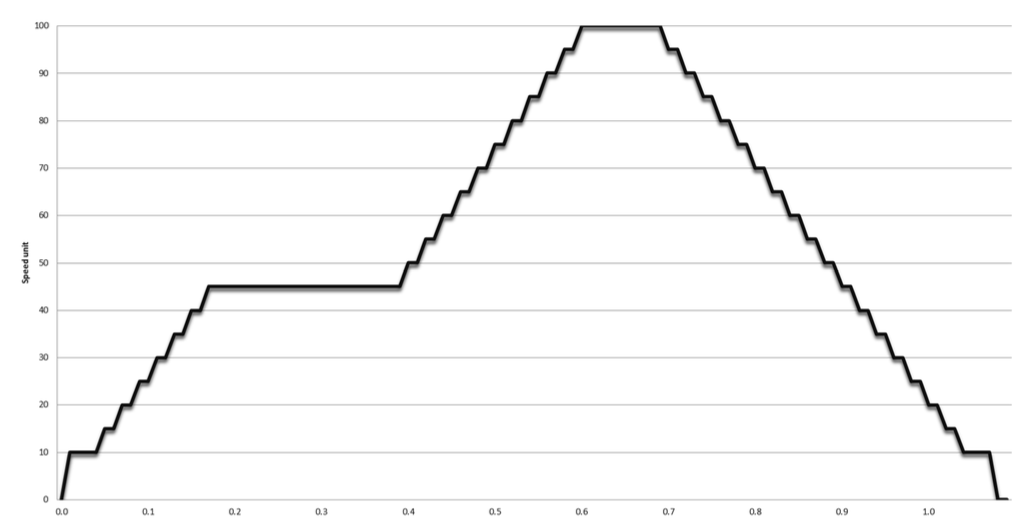
\includegraphics[width=0.5\linewidth]{files/Acceleration.png}
    \caption{Speed profile for acceleration from 0 to 45, followed by 45 to 100 and a deceleration down to 0 in speed/acceleration control mode.}
    \label{fig:acceleration}
\end{figure}

The robot listens to a set of commands defined by the manufacturer. These commands are sent via a \texttt{python} script at the desired times, both commands and times coming from a command file. A typical command file is shown in Code \ref{commandfile}.

\begin{center}
\begin{minipage}{0.9\linewidth}
    \begin{center}
\begin{lstinputlisting}[caption=\texttt{commands.txt}., label=commandfile, frame=none,numbers=none,xleftmargin=.45\textwidth]{files/commands.txt}
\end{lstinputlisting}
\end{center}
\end{minipage}
\end{center}

The first column represents the absolute time when the commands are sent (in seconds) and the second column contains the corresponding commands.
Time 0 denotes the end of a step and the beginning of the next step.
The above command script for example starts by initializing the head at time 0, followed by a forward movement at time 2.2, a turn to the right at time 6 and a stop at time 8.
The next step starts with a forward movement for 5.5 seconds, a turn to the left until time 8 and then the robot is stopped again.

The swivel wheel on the robot was found to cause instabilities in its motion. 
Their effect was first mitigated by powering off the motors completely rather than simply setting their target speed to 0 using the $s$ command. 
This approach led to some recoil in the robot's motion, however, so instead a simplified trajectory that reduces the effect of the swivel wheel was chosen. 

Figure \ref{fig:trajectory} shows the positions obtained if the robot followed the path it was given exactly, assuming it reaches its target speed (\u{0.3}{m\per s}) instantaneously, compared to the results of odometry. 
It can be clearly seen that due to communication latency and unexpected delays, the actual trajectory differs significantly from the expected one, especially when turning takes place. 
This discrepancy is not a major problem since the robot does not need to accurately attain given positions, however it does indicate the need for an external positioning system to accuractely localize the robot.

\begin{figure}
	\centering
	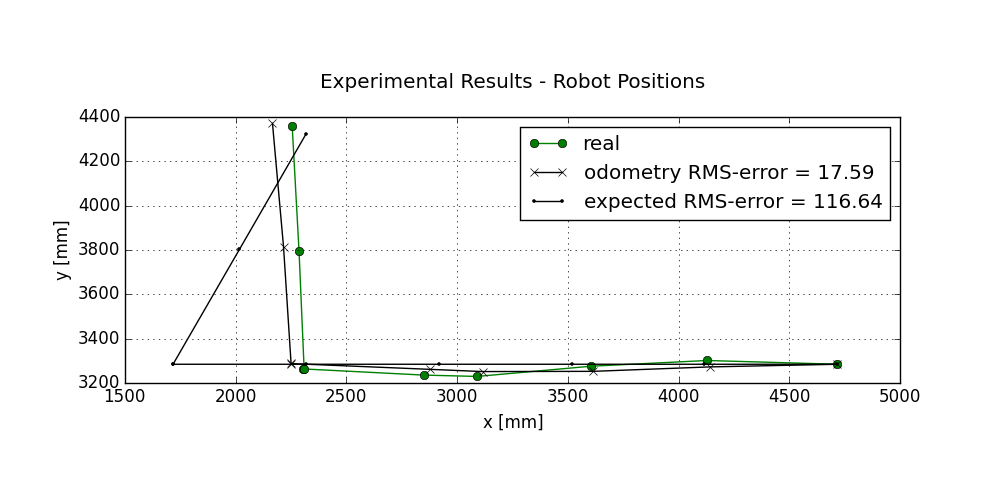
\includegraphics[width=0.8\linewidth]{files/trajectory.png} 
	\caption{Real trajectory of the robot vs. expected trajectory and trajectory estimated by odometry.}
	\label{fig:trajectory}
\end{figure}

Figure \ref{fig:trajectory} shows the positions obtained if the robot followed the path it was given exactly, assuming it reaches its target speed (\u{0.3}{m\per s}) instantaneously, compared to the results of odometry. 
It can be clearly seen that due to communication latency and unexpected delays, the actual trajectory differs significantly from the expected one, especially when turning takes place. 
This discrepancy is not a major problem since the robot does not need to accurately attain given positions, however it does show the need for an external positioning system to accuractely localize the robot.

\begin{figure}
	\centering
	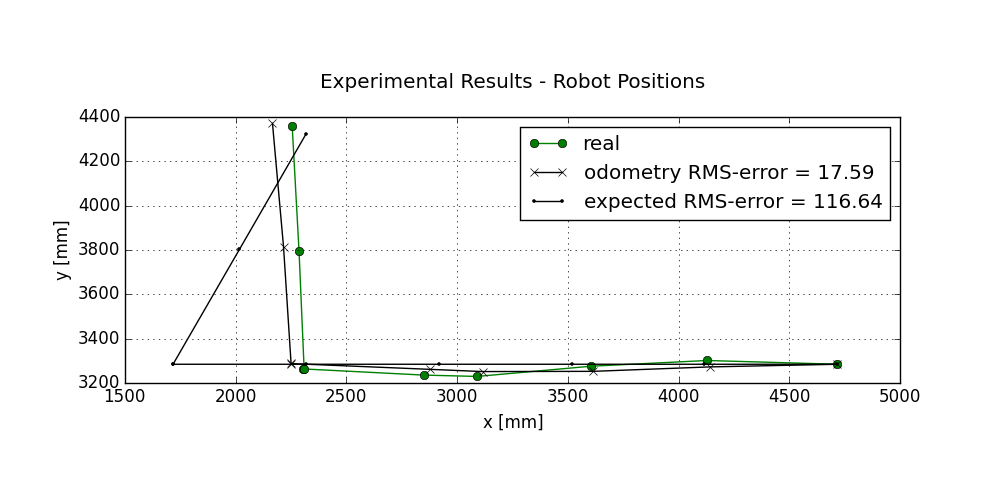
\includegraphics[width=0.8\linewidth]{files/trajectory.png} 
	\caption{Real trajectory of the robot vs. expected trajectory and trajectory estimated by odometry.}
	\label{fig:trajectory}
\end{figure}

\subsection{Odometry}

The following considerations follow from basic geometry and Borenstein \cite{Borenstein1996}.

Given the incremental encoder readings from the left and the right motor respectively ($e_{left,i},e_{right,i}$) and assuming no slip of the wheels on the ground, odometry allows to calculate the relative change in position as follows.

First of all, the odometry measurements can be converted in the trajectory length using
\begin{align}
    l_{left,i} &= \frac{2\pi R_{wheels} e_{left,i}}{N_{tot}} \\
    l_{right,i} &= \frac{-2\pi R_{wheels} e_{right,i}}{N_{tot}}.
    \label{eq:encoders} 
\end{align}
Note that the right encoder reading is inverted because of the mounting of the wheels facing in opposite directions.

Starting from a first position $\begin{bmatrix} x_i,y_i,\theta_i \end{bmatrix}$, where $\theta_i$ denotes the rotation of the robot axis with respect to the $x$ axis (see Figure \ref{fig:odometry}), the next position is obtained with the following formulas, derived from geometric considerations.

\begin{subequations}
    \begin{align}
        \theta_{i+1} &= \theta_i + \frac{l_{left,i}-l_{right,i}}{L} \\
        y_{i+1} &= y_i + R_i (\sin(\theta_{i+1})-\sin(\theta_{i})) \\
        x_{i+1} &= x_i + R_i (\cos(\theta_{i+1})-\cos(\theta_i)) \\
        \text{where} \quad R_{i} &= \frac{L}{2} \frac{l_{left,i}+l_{right,i}}{l_{left,i}-l_{right,i}}.
    \label{eq:positions}
\end{align}
\end{subequations}

$L$ is length of the robot axis or the distance between the two wheels. 
$R$ denotes the radius of the circle formed by the center of the robot axis with center $C_{i,i+1}$ (see Figure \ref{fig:odometry}).
\hspace{2em}

\begin{figure}[htb]
    \centering
    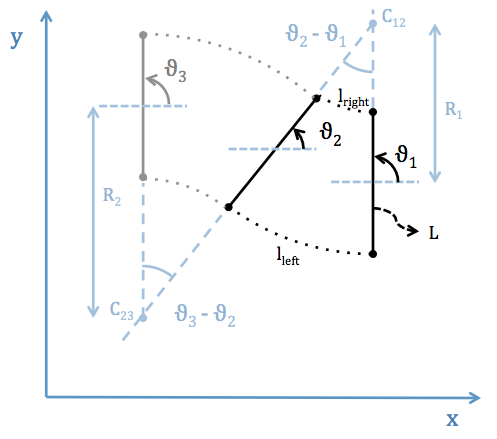
\includegraphics[width=0.7\linewidth]{files/Odometry.png}
    \caption{Geometry considerations for odometry for three example positions.}
    \label{fig:odometry}
\end{figure}
